\noindent
\textbf{Thermodynamics:
\ifthenelse{\equal{\solutions}{true}}{Examples}{Homework} for chapter 3.}\\

\begin{enumerate}

\item Show that $(\partial C_V / \partial V) = 0$ for a) an ideal gas, b) a van der Waals gas and c) a gas following $P = \frac{nRT}{V - nb}$. Assume that the following result holds:

$$\left(\frac{\partial U}{\partial V}\right)_T = T\left(\frac{\partial P}{\partial T}\right)_V - P$$

Hint: In b) and c), differentiate with respect to both temperature and volume and recall that for exact differentials the order of differentiation can be exchanged.

\ifthenelse{\equal{\solutions}{true}}{% Problem 1/3 solution
\noindent
\underline{Solution:}\\

The lecture notes give: $C_V = \left(\frac{\partial U}{\partial T}\right)_V$. Differentiate this equation with respect to volume:

$$\left(\frac{\partial C_V}{\partial V}\right)_T = \left(\frac{\partial}{\partial V}\left(\frac{\partial U}{\partial T}\right)_V\right)_T = \left(\frac{\partial}{\partial T}\left(\frac{\partial U}{\partial V}\right)_T\right)_V$$

By using the relation given in the problem, we can write this as:

$$\left(\frac{\partial C_V}{\partial V}\right)_T = \left(\frac{\partial}{\partial T}\left(\frac{\partial U}{\partial V}\right)_T\right)_V = \left(\frac{\partial\left(-P + T\left(\partial P / \partial T\right)_V\right)}{\partial T}\right)_V = T\left(\frac{\partial^2 P}{\partial T^2}\right)_V$$

Next we consider the various equations of state:

\begin{itemize}
\item[a)] Ideal gas. $P = nRT / V$ from which the second derivative of pressure (see above) is zero and therefore $\left(\frac{\partial C_V}{\partial V}\right)_T = 0$.

\item[b)] For a van der Waals gas we have: $P = \frac{nRT}{V - nb} - \frac{n^2a}{V^2}$. Differentiation of $P$ with respect to $T$ once just gives $nR / (V - nb)$. This does not depend on $T$ and hence $\left(\frac{\partial C_V}{\partial V}\right)_T = 0$.

\item[c)] Differentiation of $P$ twice with respect to $T$ again gives zero and hence $\left(\frac{\partial C_V}{\partial V}\right)_T = 0$.
\end{itemize}

\hrule\vspace{0.5cm}
}{}

\item Show that $q_{rev}$ is not a state function (i.e. $dq_{rev}$ is not exact) for a gas obeying the equation of state $P = \frac{RT}{\bar{V} - b}$, but that $d_{qrev} / T$ is. Assume a reversible process and consider only $PV$-work. Hint: you may proceed as follows:

\begin{enumerate}
\item Use the previous problem to calculate $\left(\partial U / \partial V\right)_T$.
\item Use $dU = \left(\frac{\partial U}{\partial T}\right)_VdT + \left(\frac{\partial U}{\partial V}\right)_TdV$ to calculate $dU$.
\item Use the first law of thermodynamics to get an expression for $dq$.
\item Substitute the equation of state into the above expression.
\item Apply the exactness test for differentials ($dq = M(V,T)dT + N(V,T)dV$). Use results from the previous problem to differentiate $M$ with respect to $V$.
\item Repeat the same calculation for $dq/T$.
\end{enumerate}

\ifthenelse{\equal{\solutions}{true}}{% Problem 2/3 solution
\noindent
\underline{Solution:}\\

By using the result given in the first problem, we can obtain $\left(\frac{\partial U}{\partial V}\right)_T = 0$. The total differential for $dU$ now gives $dU = \left(\frac{\partial U}{\partial T}\right)_VdT$ and hence $dU = C_VdT$. The first law of thermodynamics, $dU = dq + dw$, gives $dq = C_VdT - dw$. Considering $PV$-work, we can write: $dq = C_VdT + P_{ext}dV$. Because the process is reversible, $P_{ext} = P$ and $dq = C_VdT + PdV$. For $dq$ to be exact we should have:

$$\left(\frac{\partial C_V}{\partial V}\right)_T = \left(\frac{\partial P}{\partial T}\right)_V$$

From the first problem we know that the left hand side is zero. The right hand side, however, is not zero:

$\left(\frac{\partial P}{\partial T}\right)_V = \frac{nR}{V - nb} \ne 0$

Thus $dq$ is inexact. For $dq / T$ we have: $\frac{dq}{T} = \frac{C_V}{T}dT + \frac{P}{T}dV$. Now the exactness test gives:

$$\left(\frac{\partial C_V / T}{\partial V}\right)_T = 0\textnormal{ (}T\textnormal{ is constant)}$$
$$\left(\frac{\partial (nR / (V - nb))}{\partial T}\right)_V = 0\textnormal{ (the expression does not depend on }T\textnormal{)}$$

Thus $dq/T$ is exact.

\hrule\vspace{0.5cm}
}{}

\item An ideal gas initially at $(P_1, V_1, T_1)$ undergoes a reversible isothermal expansion to $(P_2, V_2, T_1)$ (path 1). The same change in state of the gas can be achieved by allowing it to expand adiabatically from $(P_1, V_1, T_1)$ to $(P_3, V_2, T_2)$ and then heating it at constant volume to $(P_2, V_2, T_1)$ (path 2). Note that $T_2$ has not been specified and you should find an equation that determines it. Show that the entropy change for the reversible isothermal expansion (path 1) is the same as the sum of the entropy changes in the reversible adiabatic expansion and the reversible heating (path 2). Because the two paths give the same result, it is probable that the integral is independent of path. This is not a complete proof -- why?

\ifthenelse{\equal{\solutions}{true}}{% Problem 3/3 solution
\noindent
\underline{Solution:}\\

\textbf{Path 1}: First we recall that for an ideal gas $U = \frac{3}{2} nRT$ (see lecture notes). The temperature is constant along this path and thus change in internal energy must be zero. The first law of thermodynamics now states that $\Delta UU = q_{rev} + w_{rev}$ and hence $q_{rev} = -w_{rev}$. Recall the following equation from the lecture notes:

$$w_{rev} = -nRT_1\ln\left(\frac{V_2}{V_1}\right) \Rightarrow q_{rev} = nRT_1\ln\left(\frac{V_2}{V_1}\right)$$

Using the definition of entropy gives:

$$\Delta S = \frac{q_{rev}}{T_1} = nR\ln\left(\frac{V_2}{V_1}\right)$$

\textbf{Path 2}: First consider the first segment from ($P_1$, $V_1$, $T_1$) to ($P_3$, $V_2$, $T_2$). The expansion is adiabatic (i.e. no heat exchange with the surroundings) and hence $q_{rev} = 0$. For this reason the change in entropy is also zero ($\Delta S = q_{rev} / T = 0$). The final temperature in an adiabatic expansion is determined by integrating $C_V\frac{dT}{T} = -nR\frac{dV}{V}$ (see lecture notes):

$$\int\limits_{T_1}^{T_2}\frac{C_V}{T}dT = -nR\int\limits_{V_1}^{V_2}\frac{dV}{V} = -nR\ln\left(\frac{V_2}{V_1}\right)$$

Along the second segment ($P_3$, $V_2$, $T_2$) to ($P_2$, $V_2$, $T_1$), we have a constant volume process. The lecture notes now give $dq_{rev} = C_VdT$. The definition of entropy is $dS = \frac{dq_{ref}}{T}$ and thus:

$$dS = \frac{C_VdT}{T} \Rightarrow \Delta S = \int\limits_{T_2}^{T_1}\frac{C_VdT}{T} = -\int\limits_{T_1}^{T_2}\frac{C_VdT}{T}$$

Comparison of this with the expression determining $T_2$ along the first segment, gives the final result:

$$\Delta S = nR\ln\left(\frac{V_2}{V_1}\right)$$

This is the same result that was obtained along path 1. For a complete proof of exactness, one would have to use the exactness test or consider infinitely many paths (or rather, the exactness test).

\hrule\vspace{0.5cm}
}{}

\item Water is vaporized reversibly at 100 $^\circ$C and 1.01325 bar. The heat of vaporization is 40.69 kJ mol$^{-1}$. a) What is the value of $\Delta S$ for the water? b) What is the value of $\Delta S$ for the water plus the heat reservoir at 100 $^\circ$C? The heat reservoir is thermally isolated from its surroundings.

\ifthenelse{\equal{\solutions}{true}}{% Problem 3/4 solution
\noindent
\underline{Solution:}\\

\noindent
The MO diagram is:\\
\noindent
\begin{figure}[h]
\centering
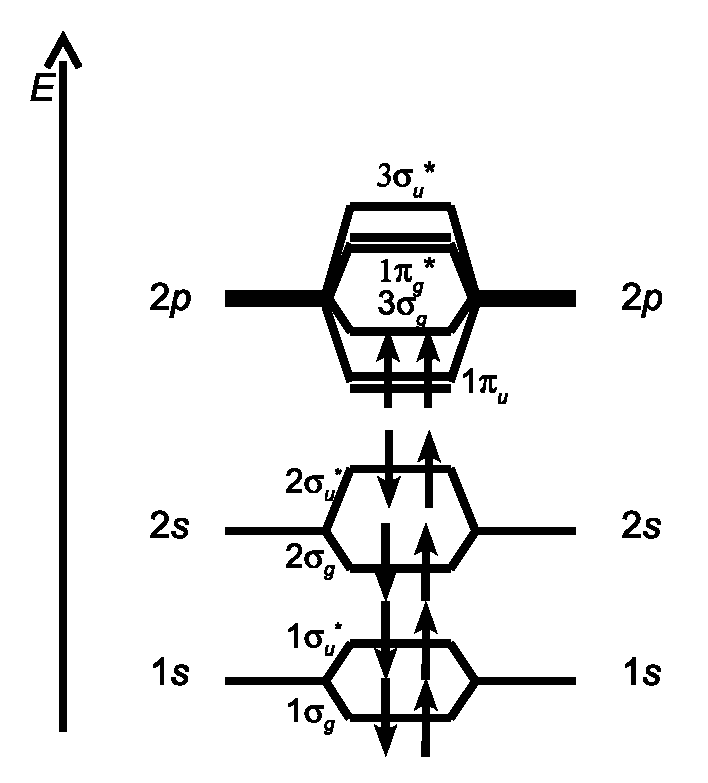
\includegraphics[scale=0.5]{b2mo}
\end{figure}

\noindent
The term symbol is $^3\Sigma_g$.\\

\hrule\vspace{0.5cm}
}{}

\item Assuming that CO$_2$ is an ideal gas, calculate $\Delta H^\circ$ and $\Delta S^\circ$ for the following process:

$$\textnormal{CO}_2(g, 298.15\textnormal{ K}, 1\textnormal{ bar}) \rightarrow \textnormal{CO}_2(g, 1000\textnormal{ K}, 1\textnormal{ bar})$$

Consider 1 mol of gas and a reversible process. Given: $\bar{C}^{\circ}_P(T) = 26.648 + 42.262 \times 10^{-3}T - 142.4 \times 10^{-7}T^2$ (units: J K$^{-1}$ mol$^{-1}$).

\ifthenelse{\equal{\solutions}{true}}{% Problem 3/5 solution
\noindent
\underline{Solution:}\\

\noindent
a) XeF is not a homonuclear diatomic molecule. Thus the atomic orbitals 
that form MOs originate from different principal quantum number levels.
The MO diagram is:\\
\newpage
\noindent
\begin{figure}[h]
\centering
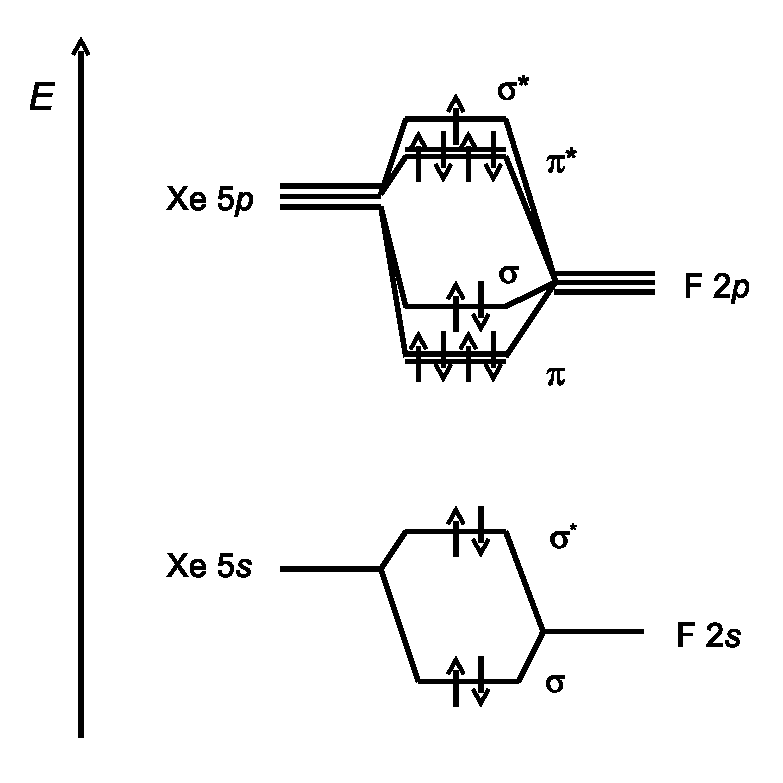
\includegraphics[scale=0.5]{xefmo}
\end{figure}

\noindent
The bond order for XeF is $(8 - 7) / 2 = 0.5$ and for XeF$^+$ $(8 - 6)
/ 2 = 1$. Thus the equilibrium bond length for XeF$^+$ is expected to be
shorter than for XeF.\\

\noindent
b) Consider the MOs of the C=C fragment:
\noindent
\begin{figure}[h]
\centering
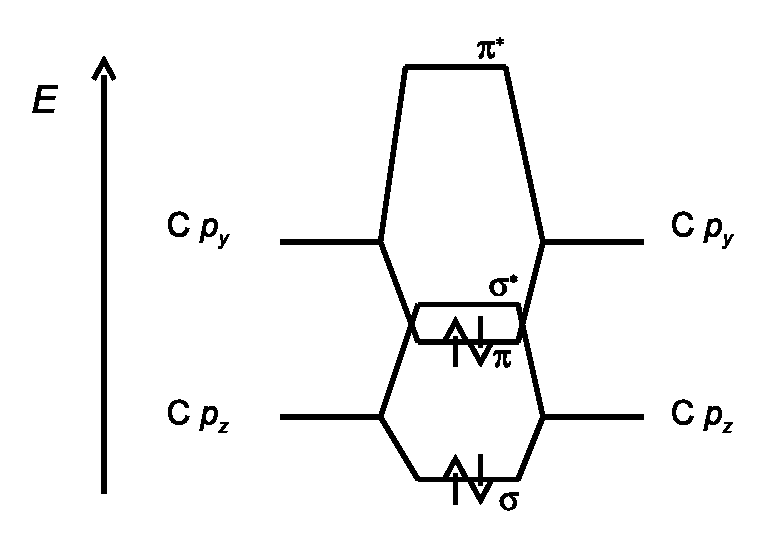
\includegraphics[scale=0.5]{ccmo}
\end{figure}

\noindent
Note that the order of the $\pi$ and $\sigma^*$ orbitals must be as shown
above. If this was not the case, the C=C fragment would not be bound!\\

\noindent
c) All the resulting bonding and antibonding orbitals become fully occupied. 
As antibonding orbitals cause more repulsion than bonding orbitals binding,
the result is no chemical binding. In general, the octet electronic
structure in atoms (e.g. rare gases) tends to lead to efficient population of the antibonding
molecular orbitals and hence they are chemically inert.\\

\hrule\vspace{0.5cm}
}{}

\item Ammonia (considered to be an ideal gas) initially at 25 $^\circ$C and 1 bar pressure is heated at constant pressure until the volume has trebled. Assume reversible process. Calculate: a) $q$ per mole, b) $w$ per mole, c) $\Delta\bar{H}$, d) $\Delta\bar{U}$, e) $\Delta\bar{S}$ given $\bar{C}_P = 25.895 + 32.999\times 10^{-3}T - 30.46\times 10^{-7}T^2$ (in J K$^{-1}$ mol$^{-1}$).

\ifthenelse{\equal{\solutions}{true}}{% Problem 6/3 solution
\noindent
\underline{Solution:}\\

Tripling of the ideal gas volume ($PV_1 = nRT_1$) leads to $T = P(3V_1) / (nRT)$, which means that the temperature will be three times higher; $T_2 = 3T_1$. Note that pressure is constant.

\begin{itemize}
\item[a)] $q = \int\limits_{T_1}^{T_2}\bar{C}_PdT = \int\limits_{298\textnormal{ K}}^{894\textnormal{ K}}\left(25.895 + 32.999\times 10^{-3}T - 30.46\times 10^{-7}T^2\right)dT = 26.4\textnormal{ kJ mol}^{-1}$.

\item[b)] $w = -P\Delta\bar{V} = -R\Delta T = -\left(8.314\textnormal{ J K}^{-1}\textnormal{ mol}^{-1}\right)\times\left(596\textnormal{ K}\right) = -4.96\textnormal{ kJ mol}$.

\item[c)] Because pressure is constant, we have $\Delta\bar{H} = q_P = 21.4\textnormal{ kJ mol}^{-1}$.

\item[d)] $\Delta\bar{U} = q + w = \left(26.4 - 4.96\right)\textnormal{ kJ mol}^{-1} = 21.4\textnormal{ kJ mol}^{-1}$.

\item[e)] $\Delta\bar{S} = \int\limits_{T_1}^{T_2}\frac{C_P}{T}dT = \int\limits_{298\textnormal{ K}}^{894\textnormal{ K}}\left(\frac{25.895}{T} + 32.999\times 10^{-3} - 30.46\times 10^{-7}T\right)dT = 46.99\textnormal{ kJ K}^{-1}\textnormal{ mol}^{-1}$.

\end{itemize}

\hrule\vspace{0.5cm}
}{}

\item Three moles of a monoatomic ideal gas expand isothermally and reversibly from 90 L to 300 L at 300 K. a) calculate $\Delta U$, $\Delta S$, $w$ and $q$ for this system, b) calculate $\Delta\bar{U}$, $\Delta\bar{S}$, $w$ per mole and $q$ per mole, c) If the expansion is carried out irreversibly by allowing the gas to expand into and evacuated container, what are the values of $\Delta\bar{U}$, $\Delta\bar{S}$, $w$ per mole and $q$ per mole?

\ifthenelse{\equal{\solutions}{true}}{% Problem 3/7 solution
\noindent
\underline{Solution:}\\

\noindent
First we construct the secular equation (matrix form) corresponding to the 
H\"uckel approximation:\\

$$\begin{pmatrix}
\alpha - E & \beta & 0\\
\beta & \alpha - E & \beta\\
0 & \beta & \alpha - E\\
\end{pmatrix}
\begin{pmatrix}
c_1\\
c_2\\
c_3\\
\end{pmatrix}
= 0$$

\noindent
Denote $x = (\alpha - E) / \beta$ and recall this set of equations
has a non-trivial solution only if the corresponding determinant is zero:

$$\begin{vmatrix}
x & 1 & 0\\
1 & x & 1\\
0 & 1 & x\\
\end{vmatrix}
= 0$$

\noindent
By expanding this determinant, we get:

$$x(x^2 - 1) - x = x^3 - 2x = x(x^2 - 2) = 0 \Rightarrow x =
\left\{
\begin{matrix}
0\\
+\sqrt{2}\\
-\sqrt{2}\\
\end{matrix}
\right.
$$

$$\Rightarrow E = \left\{\begin{matrix}
\alpha\\
\alpha - \sqrt{2}\beta\\
\alpha + \sqrt{2}\beta\\
\end{matrix}\right.
$$

\noindent
Thus we have the following energetics for the orbitals:

\begin{figure}[h]
\centering
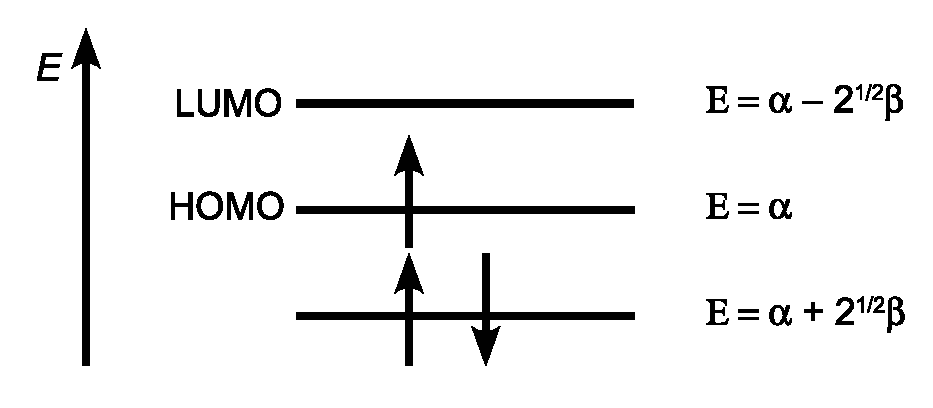
\includegraphics[scale=0.4]{huckelmo}
\end{figure}

\noindent
a) The energy difference between HOMO and LUMO orbitals is:

$$\Delta E = E_\textnormal{LUMO} - E_\textnormal{HOMO} = \alpha 
- \sqrt{2}\beta - \alpha = -\sqrt{2}\beta = -\sqrt{2}\times (-22,000
\textnormal{cm}^{-1})$$

$$\rightarrow \Delta E = 3.86 \textnormal{eV}~(320\textnormal{~nm})$$

\noindent
b) Next we calculate the coefficients $c_1, c_2$ and $c_3$ for the lowest
energy orbital:

\noindent
Here $E = (\alpha\pm\sqrt{2}\beta)$, which with $(\alpha - E)c_1 + \beta c_2 = 0$
gives $c_2 = \pm\sqrt{2}c_1$. Exactly the same way, equation
$\beta c_2 + (\alpha - E)c_3 = 0$ gives $c_2 = \pm\sqrt{2}c_3$.
Finally, normalization gives:
$c_1^2 + c_2^2 + c_3^2 = 1$ $\Rightarrow c_1^2 + (\pm\sqrt{2}c_1)^2
+ c_1^2 = 4c_1^2 \Rightarrow c_1 = \frac{1}{2}$ and by considering
$c_3$ the same way, we also get $c_3 = \frac{1}{2}$.\\

\noindent
Thus we have:

$$E = \alpha + \sqrt{2}\beta~\textnormal{with}~c_1 = \frac{1}{2},
c_2 = \frac{1}{\sqrt{2}}, c_3 = \frac{1}{2}$$
$$E = \alpha - \sqrt{2}\beta~\textnormal{with}~c_1 = \frac{1}{2},
c_2 = -\frac{1}{\sqrt{2}}, c_3 = \frac{1}{2}$$

\noindent
For $E = \alpha$, we have: $c_1 = \frac{1}{\sqrt{2}}, c_2 = 0, c_3 
= -\frac{1}{\sqrt{2}}$.\\

\noindent
The electron density on atom 1 can be obtained by squaring the atomic
basis function coefficients and weighing this by the number of electrons
on that orbital:\\

\noindent
Atom 1 ($i = 1$): $\sum_{j=1}^{3}|c_i^j|^2n_j = 
\left(\frac{1}{2}\right)^2\times 2 + \left(\frac{1}{\sqrt{2}}\right)^2
\times 1 + \left(\frac{1}{2}\right)^2\times 0 = 1$.\\
Atom 2 ($i = 2$): $\sum_{j=1}^{3}|c_i^j|^2n_j = 
\left(\frac{1}{\sqrt{2}}\right)^2\times 2 + 0^2
\times 1 + \left(-\frac{1}{\sqrt{2}}\right)^2\times 0 = 1$.\\
Atom 3 ($i = 3$): $\sum_{j=1}^{3}|c_i^j|^2n_j = 
\left(\frac{1}{2}\right)^2\times 2 + \left(-\frac{1}{\sqrt{2}}\right)^2
\times 1 + \left(\frac{1}{2}\right)^2\times 0 = 1$.\\

\noindent
The total charge (three $\pi$ electrons) is distributed evely to all three
atoms and therefore the partial charges on carbon atoms are equal.\\

\noindent
The bond orders can be valuated as follows:\\

\noindent
Bond between atoms 1 and 2 ($i = 1$ and $j = 2$):\\
$$\sum_{k=1}^{N_{MO}}c_i^k c_j^k n_k = 
\left(\frac{1}{2}\right)\left(\frac{1}{\sqrt{2}}\right)\times
2 + \left(\frac{1}{\sqrt{2}}\right)\times 0\times 1 
+ \left(\frac{1}{2}\right)\left(-\frac{1}{\sqrt{2}}\right)\times 0 
= \frac{1}{\sqrt{2}}$$
Bond between atoms 2 and 3 ($i = 2$ and $j = 3$):\\
$$\sum_{k=1}^{N_{MO}}c_i^k c_j^k n_k = 
\left(\frac{1}{\sqrt{2}}\right)\left(\frac{1}{2}\right)\times
2 + 0\times\left(-\frac{1}{\sqrt{2}}\right)\times 1
+ \left(-\frac{1}{\sqrt{2}}\right)\left(\frac{1}{2}\right)\times 0 
= \frac{1}{\sqrt{2}}$$

\noindent
The bond order is less than one ($\approx 0.707$), which indicates that
the bond is not very strong.\\

\hrule\vspace{0.5cm}
}{}

\item A monoatomic ideal gas at 298 K expands isothermally from a pressure of 10 bar to 1 bar. What are the values of $w$ per mole, $q$ per mole, $\Delta\bar{U}$, $\Delta\bar{S}$ in the following cases? a) The expansion is reversible, b) The expansion is free (irreversible), (c) The gas and its surroundings form an isolated system, and the expansion is reversible and d) The gas and its surroundings form an isolated system, and the expansion is free (irreversible).

\ifthenelse{\equal{\solutions}{true}}{% Problem 8/3 solution
\noindent
\underline{Solution:}\\

\begin{itemize}

\item[a)] This is a reversible process and constant temperature implies that $\Delta\bar{U} = 0$. Also the enthalpy change for an ideal gas depends only on temperature $\Delta\bar{H} = 0$. By using the 1st law and the expression for reversible expansion (see lecture notes), we get:

$$w_{rev} = -RT\ln\left(\frac{V_2}{V_1}\right) = -RT\ln\left(\frac{P_2}{P_1}\right) = - q_{rev}$$

By plugging in the values, we get $w_{rev} = -5.71$ kJ mol$^{-1}$ and $q_{rev} = 5.71$ kJ mol$^{-1}$. Now the definition of entropy gives the entropy change:

$$\Delta\bar{S} = \frac{q_{rev}}{T} = 19.1\textnormal{ J K}^{-1}\textnormal{ mol}^{-1}$$

\item[b)] Irreversible process (free expansion). No external pressure -- no work done ($w = 0$). Thus by the first law $q = 0$ (i.e. no heat exchanged with the surroundings) since $\Delta\bar{U} = 0$ and $\Delta\bar{H} = 0$. Entropy depends only on the endpoints of the path and hence $\Delta\bar{S} = \frac{q_{rev}}{T} = 19.1\textnormal{ J K}^{-1}\textnormal{ mol}^{-1}$, where $q_{rev}$ is from part a). Note that only reversible paths can be used in calculating entropy!

\item[c)] Isolated system, which here means that ``system + surroundings'' is isolated from the rest of the world. For a reversible process we have $dS_{tot} = dS_{syst} + dS_{surr} = 0$. For the system we have:

$$dS_{syst} = \frac{dq_{rev}}{T}\textnormal{ and for the surroundings }dS_{surr} = -\frac{dq_{rev}}{T}$$

Since temperature is constant, $\Delta U = 0$ and $\Delta H = 0$. Therefore:

$$q_{rev} = -w = RT\ln\left(\frac{P_2}{P_1}\right)\textnormal{ (from previous calculations)}$$

Thus $\Delta S_{syst} = R\ln(P_2/P_1$) and $\Delta S_{surr}  = -R\ln(P_2/P_1)$. Thus the total change of entropy (system + surroundings) is zero. Also $q_{tot} = q_{sys} + q_{surr} = RT\ln(P_2/P_1) - RT\ln(P_2/P_1) = 0$. For the same reason, the total work $w_{tot} = w_{sys} + w_{surr} = 0$. Note that the system + surroundings is isolated from the rest of the world and therefore the total change in heat ($q_{tot}$) and work ($w_{tot}$) must clearly be zero.

\item[d)] If we want to calculate the entropy change for the system, we need a reversible path for the calculation. Above this was done: $\Delta S_{syst} = R\ln(P_2/P_1)$. In free expansion, no work is done, $w_{sys} = 0$ (and $w_{surr} = 0$). Since $\Delta U = w_{sys} + q_{sys}$ and $\Delta U = 0$, $q_{sys} = 0$ as well (also then $q_{surr} = 0$). Thus the system is not interacting with the surroundings at all in this process. This means that the entropy of the surroundings does not change either, $\Delta S_{surr} =
0$. The total entropy is then $\Delta S_{tot} = \Delta S_{syst} + \Delta S_{surr} = R\ln(P_2/P_1) = 19.1$ J K$^{-1}$ mol$^{-1}$.

\end{itemize}

\hrule\vspace{0.5cm}
}{}

\item One mole of gas A at 1 bar and one mole of gas B at 2 bar are separated by a partition and surrounded by a heat reservoir (i.e. the temperature is constant). When the partition is withdrawn, how much does the entropy change? Both gases behave according to the ideal gas law. Hint: consider the calculation in three steps: (I) the initial entropy difference from standard state, (II) change in entropy due to expansion/compression of gases at constant temperature and finally (III) entropy change due to mixing of the gases.

\ifthenelse{\equal{\solutions}{true}}{% Problem 9/3 solution
\noindent
\underline{Solution:}\\

Note that the pressures of the two gases are different and thus the results in the lecture notes cannot be directly applied.

\begin{enumerate}

\item[I] The initial (i.e. before mixing) entropies for the gases are:

$$S_A = S_A^\circ - nR\ln\left(\frac{P_A^{ini}}{P_A^\circ}\right) = S_A^\circ - nR\ln\left(\frac{1\textnormal{ bar}}{1\textnormal{ bar}}\right) = S_A^\circ$$
$$S_B = S_B^\circ - nR\ln\left(\frac{P_B^{ini}}{P_B^\circ}\right) = S_B^\circ - nR\ln\left(2\right)$$

\item[II] Let both gases expand from their initial pressures to the final pressure at constant temperature. This changes entropy of both gases according to:

$$S_A = S_A^\circ - nR\ln\left(\frac{P_{total}}{P_A^\circ}\right)\textnormal{ and }S_B = S_B^\circ - nR\ln\left(\frac{P_{total}}{P_B^\circ}\right)$$

where $P_{total}$ is the final pressure after mixing. The final volume after mixing is:

$$V_{total} = V_A + V_B = \frac{nRT}{P_A} + \frac{nRT}{P_B} = \frac{nRT}{P_A} + \frac{nRT}{2P_A} = \frac{3nRT}{2P_A}$$

The total pressure after mixing is then:

$$P_{total} = \frac{2nRT}{V_{total}} = \frac{4}{3}P_A = \frac{4}{3}\textnormal{ bar}$$

The entropy change due to expansion for both gases is:

$$S_A = S_A^\circ - nR\ln\left(\frac{4}{3}\right)\textnormal{ and } S_B = S_B^\circ - nR\ln\left(\frac{4}{3}\right)$$

Combining 1 and 2, we have: $\Delta S_A = -n_AR\ln\left(\frac{4}{3}\right)$ and $\Delta S_B = -n_BR\left(\ln\left(\frac{4}{3}\right) - \ln(2)\right)$.

\item[III] Finally we must include the entropy change due to mixing ($n = 1$):

$$\Delta_{mix} S = -R\ln\left(\frac{1\textnormal{ mol}}{2\textnormal{ mol}}\right) - R\ln\left(\frac{1\textnormal{ mol}}{2\textnormal{ mol}}\right) = -2R\ln\left(\frac{1}{2}\right)$$

The total entropy change is then (``1 + 2 + 3''):

$$\Delta S_{total} = \Delta S_A + \Delta S_B + \Delta S_{mix} = -2R\ln\left(\frac{4}{3}\right) + R\ln(2) - 2R\ln\left(\frac{1}{2}\right)$$
$$ = 12.51\textnormal{ J K}^{-1}\textnormal{ mol}^{-1}$$

\end{enumerate}

\hrule\vspace{0.5cm}
}{}

\item Calculate the change in molar entropy of aluminum that is heated from 600 $^\circ$ to 700 $^\circ$C. The melting point of aluminum is 660 $^\circ$C, the heat of fusion is 393 J g$^{-1}$ (the molar mass for aluminum is 27 g mol$^{-1}$), and the heat capacities at constant pressure of the solid and the liquid may be taken as 31.8 J K$^{-1}$ mol$^{-1}$ and 34.4 J K$^{-1}$ mol$^{-1}$ (independent of temperature), respectively.

\ifthenelse{\equal{\solutions}{true}}{% Problem 10/3 solution
\noindent
\underline{Solution:}\\

Note that 600 $^\circ$C is 873 K, 660 $^\circ$C is 933 K, and 700 $^\circ$C is 973 K. Use the following equation (see lecture notes):

$$\Delta\bar{S} = \int\limits_{T_{initial}}^{T_{fusion}}\frac{C_P(s)}{T}dT + \frac{\Delta H_{fusion}}{T_{fusion}} + \int\limits_{T_{fusion}}^{T_{final}}\frac{C_P(l)}{T}dT$$

$$= C_P(s)\ln\left(\frac{T_{fusion}}{T_{initial}}\right) + \frac{\Delta H_{fusion}}{T_{fusion}} + C_P(l)\ln\left(\frac{T_{final}}{T_{fusion}}\right)$$

$$= (31.8\textnormal{ J K}^{-1}\textnormal{ mol}^{-1})\ln\left(\frac{933\textnormal{ K}}{873\textnormal{ K}}\right) + \frac{(27\textnormal{ g mol}^{-1})(393\textnormal{ J g}^{-1})}{933\textnormal{ K}}$$

$$ + (34.3\textnormal{ J K}^{-1}\textnormal{ mol}^{-1})\ln\left(\frac{973\textnormal{ K}}{933\textnormal{ K}}\right) = 19.92\textnormal{ J K}^{-1}\textnormal{ mol}^{-1}$$

\hrule\vspace{0.5cm}
}{}

\item Steam is condensed at 100 $^\circ$C, and the water is cooled to 0 $^\circ$C and frozen to ice. What is the molar entropy change of the water? Consider that the average specific heat of liquid water is 4.2 J K$^{-1}$ g$^{-1}$ (the molar mass of water is 18.016 g mol$^{-1}$). The enthalpy of vaporization at the boiling point and the enthalpy of fusion at the freezing point are 2258.1 J g$^{-1}$ and 333.5 J g$^{-1}$, respectively.

\ifthenelse{\equal{\solutions}{true}}{% Problem 11/3 solution
\noindent
\underline{Solution:}\\


Use the same cycle as in the previous problem (note that the cycle goes from high temperature to low temperature and thus the signs are reversed!):

$$\Delta\bar{S} = -\frac{\Delta H_{vap}}{T_{vap}} - \int\limits_{273.15\textnormal{ K}}^{373.15\textnormal{ K}}\frac{C_P(l)}{T}dT - \frac{\Delta H_{fus}}{T_{fus}} = -\frac{\left(2258.1\textnormal{ J g}^{-1}\right)\left(18.016\textnormal{ g mol}^{-1}\right)}{373.15\textnormal{ K}}$$

$$-\left(4.2\textnormal{ J K}^{-1}\textnormal{ mol}^{-1}\right)\times\left(18.016\textnormal{ g mol}^{-1}\right)\times\ln\left(\frac{373.15\textnormal{ K}}{273.15\textnormal{ K}}\right)$$

$$ - \frac{\left(333.5\textnormal{ J g}^{-1}\right)\left(18.016\textnormal{ g mol}^{-1}\right)}{273.15\textnormal{ K}} = -154.4\textnormal{ J K}^{-1}\textnormal{ mol}^{-1}$$

\hrule\vspace{0.5cm}
}{}

\item Calculate the increase in the molar entropy of nitrogen when it is heated from 25 $^\circ$C to 1000 $^\circ$C at constant pressure with: $\bar{C}_P = 26.9835 + 5.9622 \times 10^{-3}T - 3.377 \times 10^{-7}T^2$ in J K$^{-1}$ mol$^{-1}$.

\ifthenelse{\equal{\solutions}{true}}{% Problem 12/3 solution
\noindent
\underline{Solution:}\\

Nitrogen is gaseous in the temperature range. The entropy change is then given by:

$$\Delta\bar{S} = \int\limits_{298.15\textnormal{ K}}^{1273.15\textnormal{ K}}\frac{C_P(g)}{T}dT$$ 
$$= \sijoitus{298.15\textnormal{ K}}{1273.15\textnormal{ K}}\left(26.9835\ln(T) + 5.9622\times 10^{-3}T - \frac{3.377\times 10^{-7}}{2}T^2\right)$$
$$= 44.73\textnormal{ J K}^{-1}\textnormal{ mol}^{-1}$$

\hrule\vspace{0.5cm}
}{}

\end{enumerate}
